\documentclass[../TG_magistrsko_delo_sections.tex]{subfiles}
\graphicspath{{\subfix{../images/}}}

\begin{document}
V tem poglavju bomo podali definicijo Štefanovega zaporedja točk. Pokazali bomo, da te točke določajo intervale, s pomočjo katerih lahko zapišemo relacije pokritja in ustrezne zanke, ki zagotavljajo obstoj periodičnih točk. 
Če $f$-orbita vsebuje samo eno točko, je ta točka fiksna točka funkcije $f$. Perioda te točke je 1, kar je zadnji člen ureditve Šarkovskega in pri tej orbiti nimamo kaj dokazovati. Zato bomo obravnavali samo orbite oziroma cikle, ki vsebujejo vsaj dve točki. Naj bo $m \geq 2$ in $\mathcal{O}$ $m$-cikel zvezne funkcije $f$. Preden definiramo Štefanovo zaporedje, moramo spoznati nekaj pojmov. 

\begin{definicija}
Za točki $x$ in $y$ iz cikla $\mathcal{O}$  rečemo, da točka $x$ leži desno od točke $y$, če velja $x < y$. Naj bo $p$ najbolj desna točka $m$-cikla $\mathcal{O}$, za katero je $f(p) > p$ in $q\in \mathcal{O}$ prva točka desno od p. Center $c$ cikla $\mathcal{O}$ definiramo kot $c=\frac{p+q}{2}$. Za vsako točko $x \in \mathcal{O}$ označimo množico točk iz cikla $\mathcal{O}$, ki ležijo v zaprtem intervalu omejenim z $x$ in $c$, z $\mathcal{O}_x$. Natančneje, $\mathcal{O}_x = \mathcal{O} \cap [x, p]$, če je $x \leq p$ in  $\mathcal{O}_x = \mathcal{O} \cap [q, x]$, če je $x \geq q$. Pravimo, da točka $x \in \mathcal{O}$ menja strani, če točka $c$ leži med točkama $x$ in $f(x)$. Torej velja $x < c < f(x)$ ali $f(x) < c < x$.
\end{definicija}
Poglejmo si definicijo Štefanovega zaporedja.

\begin{definicija}\label{def:stef}
Iz $m$-cikla $\mathcal{O}$ izbrane točke $x_0, x_1, \dots, x_n$ tvorijo Štefanovo zaporedje, če je:

\begin{enumerate}[label={(Š\arabic*)}]\label{def:stef-zap}
    \item $\{x_0, x_1\} = \{p, q\}$, \label{eq:š1}
    \item točke $x_0, x_1, \dots, x_n$ ležijo alternirajoče na levi oziroma desni strani točke $c$, \label{eq:š2}
    \item zaporedji 
    $\left \{ x_{2j} \right \}_{j=0}^{\left \lfloor \frac{n}{2} \right \rfloor}$ 
    in
    $\left \{ x_{2j+1} \right \}_{j=0}^{\left \lfloor \frac{n}{2} \right \rfloor}$ sta strogo monotoni in se oddaljujeta od točke $c$, \label{eq:š3}
    \item če je $0\leq j \leq n-1$, potem $x_j$ menja strani in $x_{j+1} \in \mathcal{O}_{f(x_j)}$,\label{eq:š4}
    \item točka $x_n$ ne menja strani. \label{eq:š5}
\end{enumerate}
\end{definicija}

\begin{opomba}\label{op:štefzap}
Štefanovo zaporedje dobimo tako, da iz množice $m$ točk, ki tvorijo $\mathcal{O}$-cikel izberemo $n+1$ točk, ki zadoščajo zgornjim pogojem. 
Pogoj $x_{j+1} \in \mathcal{O}_{f(x_j)}$ v~\ref{eq:š4} pomeni, da je točka $x_{j+1}$ bližje centru kot slika $f(x_j)$ točke $x_j$. Velja ena od neenakosti: $c < x_{j+1} \leq f(x_j)$ ali $f(x_j) \leq x_{j+1} < c$. Pogoja ~\ref{eq:š2} in~\ref{eq:š3} zagotavljata, da so točke $x_0, x_1, \dots, x_n$ paroma različne. Če sledimo točkam na način, ki je opisan v primeru~\ref{primer3}, dobimo spiralo, zato za točke, ki ustrezajo pogojema ~\ref{eq:š2} in~\ref{eq:š3} rečemo, da se spiralno oddaljujejo od centra $c$. Ker lahko pri izbiri točk iz cikla $\mathcal{O}$ kakšno točko izpustimo, je število $n+1$ izbranih točk manjše ali enako številu vseh točk v $\mathcal{O}$-ciklu. Velja torej neenakost $n+1 \leq m$. Če se vrnemo na primere iz prejšnjega poglavja, lahko vidimo, da v primerih~\ref{primer1}, \ref{primer2} in \ref{primer4} Štefanovo zaporedje sestavljajo vse točke $\mathcal{O}$-cikla. V primeru~\ref{primer3} pa dve točki $\mathcal{O}$-cikla ne nastopata v Štefanovem zaporedju.
\end{opomba}

\begin{trditev}\label{trd:zap-cikel}
Predpostavimo, da $m$-cikel $\mathcal{O}$ vsebuje Štefanovo zaporedje. Če je $l \triangleleft m$, potem funkcija $f$ vsebuje $\mathcal{O}$-vsiljeno elementarno $l$-zanko $\mathcal{O}$-intervalov in posledično tudi periodično točko s periodo $l$.
\end{trditev}

Pri danem Štefanovem zaporedju $x_0, x_1, \dots, x_n$ definiramo intervale $I_0, I_1, \dots, I_{n-1}$ na  nasledni način: Za $1 \leq j < n$ najkrajši $\mathcal{O}$-interval, ki vsebuje točke $x_0$, $x_1$ in $x_j$, označimo z $I_j$, medtem ko z $I_0$ označimo $\mathcal{O}$-interval s krajišči $x_{n-2}$ in $x_n$. Iz lastnosti~\ref{eq:š2} lahko sklepamo, da je $\interior(I_0) \cap I_j = \emptyset$ za vsak $j \in \{1, 2, \dots, n-1\}$.

\begin{trditev}\label{trd:pokritja}
Za intervale izbrane na zgoraj opisan način veljajo naslednje relacije pokritja:
\begin{enumerate}[label={(\arabic*)}]
\item $I_1 \to I_1$ in $I_0 \to I_1$,\label{trd:pokritja1}
\item $I_1 \to I_2 \to \cdots \to I_{n-1} \to I_0$,\label{trd:pokritja2}
\item $I_0 \to I_{n-1}, I_{n-3}, I_{n-5} \dots $\label{trd:pokritja3}
\end{enumerate}
Zaradi boljše predstave ponazorimo relacije pokritja na sliki~\ref{fig:nkotnik}.
\end{trditev}

\begin{figure}[h]
  \centering
  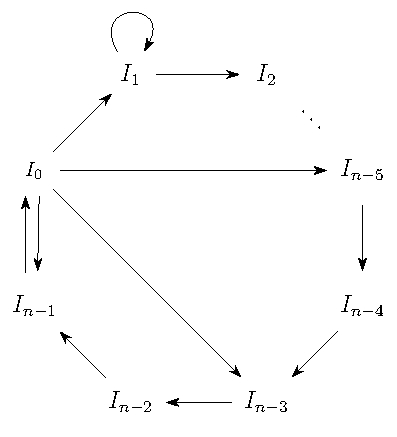
\includegraphics{graph_n.pdf}
% \caption[caption za v kazalo]{Dolg caption pod sliko}
  \caption[Primer vektorske slike.]{Relacije pokritja v trditvi~\ref{trd:pokritja} lahko prikažemo z grafom.}
  \label{fig:nkotnik}
\end{figure}

\begin{proof}[Dokaz trditve~\ref{trd:pokritja}]
Dokazovali bomo vsako točko posebej. 

Pri dokazu točke~\ref{trd:pokritja1} bomo dokazali še močnejšo trditev, ki nam bo v pomoč tudi pri dokazu druge točke. Pokazali bomo, da za vsak $j = 0, 1, \dots, n-1$ velja relacija pokritja $I_j \to I_1$.  Za dokaz je dovolj, če se prepričamo, da za vsak $j=0, 1, \dots, n-1$ množica $f(I_j)$ vsebuje točki $x_0$ in $x_1$. To je res, saj posledica~\ref{pos:vmesnavrednost} zagotavlja, da so v množici $f(I_j)$ vsebovane tudi vse točke iz intervala $(x_0, x_1)$. V primeru intervala $I_0 = [x_n, x_{n-2}]$ ugotovimo, da obe krajišči $I_0$ ležita na isti strani točke $c$. Lastnost \ref{eq:š4} pove, da krajišče $x_{n-2}$ menja strani, medtem ko lastnost~\ref{eq:š5} pravi, da točka $x_n$ ne menja strani, zato točki $f(x_n)$ in $f(x_{n-2})$ ležita na nasprotnih straneh točke $c$. V primeru intervala $I_j$ za $j = 1, 2, \dots, n-1$ iz lastnosti~\ref{eq:š2} izvemo, da krajišči intervala $I_j$ ležita na nasprotnih straneh točke $c$. Lastnost~\ref{eq:š4} pove, da obe krajišči menjata strani. Torej za vsak $j=0, 1, \dots, n-1$ interval $f(I_j)$ vsebuje točke cikla $\mathcal{O}$, ki ležijo na obeh straneh centra $c$. Zagotovo vsebuje točki $x_0$ in $x_1$ in zato tudi interval $I_1$.

Naj bo $j$ tako naravno število, za katerega velja $1 \leq j \leq n-1$. Želimo pokazati, da množica $f(I_j)$ vsebuje interval $I_{j+1}$. Vemo že, da interval $f(I_j)$ vsebuje točki $x_0$ in $x_1$. Za dokaz točke~\ref{trd:pokritja2} moramo pokazati samo še vsebovanost točke $x_{j+1}$ v množici $f(I_j)$. Podobno kot prej posledica~\ref{pos:vmesnavrednost} zagotavlja, da je v množici $f(I_j)$ vsebovan celoten interval $I_{j+1}$. V množici $f(I_j)$ so vsebovane točke $x_0, x_1$ in $f(x_j)$, zato je v tej množici vsebovana tudi množica točk $\mathcal{O}_{f(x_j)}$. Iz lastnosti~\ref{eq:š3} ugotovimo točka $x_{j+1}$ leži v množici $\mathcal{O}_{f(x_j)}$, zato velja $x_{j+1} \in \mathcal{O}_{f(x_j)} \subseteq f(I_j)$. Torej je interval $I_{j+1}$ res vsebovan v množici $f(I_j)$.

Za dokaz točke~\ref{trd:pokritja3} moramo pokazati, da je za vsako liho število $1 \leq d \leq n$ interval $I_{n-d}$ vsebovan v množici $f(I_0)$.  
Ker že vemo, da $f(I_0)$ vsebuje točki $x_0$ in $x_1$, preostane za dokazati še, da vsebuje točko $x_{n-d}$. Zaradi lastnosti~\ref{eq:š2} leži točka $x_{n-d}$ na drugi strani točke $c$ kot točki $x_{n-2}$ in $x_n$. Iz lastnoti~\ref{eq:š3} sklepamo, da je točka $x_{n-1}$ bolj oddaljena od točke $c$, kot točka $x_{n-d}$ za liho število $3 \leq d \leq n$, zato vsak interval, ki vsebuje točke $x_0, x_1$ in $x_{n-1}$, vsebuje tudi točko $x_{n-d}$. Pokazati moramo samo še, da množica $f(I_0)$ vsebuje točko $x_{n-1}$. Pri lastnosti~\ref{eq:š4} namesto $j$ pišemo $n-2$ in dobimo vsebovanost $x_{n-1} \in \mathcal{O}_{f(x_{n-2})}$. To pomeni, da je točka $f(x_{n-2}$ vsaj tako oddaljena od točke $c$, kot točka $x_{n-1}$. Dokazali smo, da množica $f(I_0)$ vsebuje točke $x_0, x_1$ in $x_{n-1}$, zato vsebuje vse intervale $x_{n-1}, x_{n-3}, x_{n-5}, \dots$
\end{proof}


\begin{proof}[Dokaz trditve~\ref{trd:zap-cikel}]
Naj veljajo predpostavke v trditvi~\ref{trd:zap-cikel}. Radi bi pokazali, da ima funkcija $f$ za vsako naravno število $l$, za katero velja $l\triangleleft m$ točko periode $l$. Dokaz bomo razdelili na tri dele. Najprej bomo dokazali izrek za liha števila manjša od $m$, potem za soda števila manjša od $m$ in na koncu še za vsa števila večja od $m$.
Pri dokazu si bomo pomagali z naslednjimi zankami, ki jih preberamo s slike~\ref{fig:nkotnik}:
\begin{enumerate}[label={(Z\arabic*)}]
\item $I_1 \to I_1$,\label{eq:z1}
\item$I_0\to I_{n-(l-1)} \to I_{n-(l-2)} \to \cdots \to I_{n-2} \to I_{n-1} \to I_0$ za sodo število $l \leq n$,\label{eq:z2}
\item $I_0\to\underbrace{I_1 \to I_1 \to \cdots  \to I_1}_{l - n +1 \text{ ponovitev intervala } I_1} \to I_2 \to \cdots \to I_{n-1} \to I_0 $ za $l \geq n$.\label{eq:z3}
\end{enumerate}
Edino liho število $l$ manjše od $m$, za katerega lahko velja $l\triangleleft m$ je število 1. Za $l=1$ uporabimo zanko~\ref{eq:z1}, ki je zanka dolžine 1 in zato elementarna. Torej obstaja točka periode 1 v intervalu $I_1$.

Naravno število  $1<l \leq m$ je lahko v relaciji $l \triangleleft m$ samo, če je sodo. Za vsako sodo število $l \leq n$ uporabimo zanko~\ref{eq:z2}.
Iz konstrukcije intervalov $I_0, I_1, \dots, I_n$ vemo, da je notranjost intervala $I_0$ disjunktna z intervali $I_{n-(l-1)}, I_{n-(l-2)}, \dots, I_{n-2}, I_{n-1}$. Krajišči intervala $I_0$ imata periodo $m$ in zato ne moreta sledit zanki~\ref{eq:z2}, katere dolžina je manjša od $m$. Z uporabo leme~\ref{lem:element} ugotovimo, da je zanka~\ref{eq:z2} elementarna, zato obstaja točka iz $I_0$, ki ima periodo $l$.

V primeru, ko je $l >n$, si pomagamo z $l$-zanko~\ref{eq:z3}.
Če je $l=m$, potem lahko izberemo poljubno točko iz cikla $\mathcal{O}$, saj imajo vse točke iz cikla $\mathcal{O}$ periodo $m$. Predpostavimo, da je $l \neq m$. Podobno kot v prejšnjem primeru je notranjost intervala $I_0$ disjunktna z intervali $I_1, I_2, \dots, I_{n-1}$. Pri dokazu, da kraišči intervala $I_0$ ne sledita zanki~\ref{eq:z3}, bomo obravnavali dva primera. Če velja $n<l<m$, potem krajišči intervala ne moreta slediti zanki~\ref{eq:z3}, saj je njena dolžina manjša od $m$, perioda krajišč intervala $I_0$ pa je $m$. Če je $l >m$ si pogledamo, koliko ponovitev intervala $I_1$ nastopa v zanki~\ref{eq:z3}. Število $l$ je večje od števila $m$. Iz opombe~\ref{op:štefzap} lahko preberemo, da je število $m$ večje od števila $n+1$ in naredimo naslednje ocene:
$$l-n+1>m-n+1 \geq n+1-n+1 = 2.$$
Število ponovitev intervala $I_1$ je večje od 2, kar pomeni, da se v zanki~\ref{eq:z3} interval $I_1$ pojavi vsaj trikrat. Ker za nobeno točko iz cikla $\mathcal{O}$ v intervalu $I_1$ ne ležijo tri zaporedne iteracije, tudi krajišča intervala $I_0$ ne morejo slediti zanki~\ref{eq:z3}. S pomočjo leme~\ref{lem:element} sklepamo, da je zanka~\ref{eq:z3} elementarna, kar zagotavlja obstoj točke iz intervala $I_0$, ki ima periodo $l$.
\end{proof}

Pri pozornem spremljanju dokaza opazimo, da smo dokazali močnejšo trditev.

\begin{trditev}\label{trd:posplositev}
Če $m$-cikel $\mathcal{O}$ vsebuje Štefanovo zaporedje dolžine $n<m-1$, potem ima obstaja periodična točka s periodo 1 (sledi iz zanke~\ref{eq:z1}), točka s sodo periodo $l \leq n$ (sledi iz zanke~\ref{eq:z2}) in točka s periodo $l \geq n$ (sledi iz zanke~\ref{eq:z3}).
\end{trditev}

S pomočjo trditve~\ref{trd:posplositev} lahko dokažemo tudi obstoj nekaterih periodo $l$, kjer je $l \triangleright m$. 
%Vsakič, ko iz $m$-cikla $\mathcal{O}$ izberemo $n+1$ točk, ki tvorijo štefanovo zaporedje 
Ekstremen primer dobimo, če je točka $q$ največja točka intervala $\mathcal{O}$ in točka $f(q)$ najmanjša točka intervala $\mathcal{O}$.  V tem imamo cikel oblike:
\tikz{
\tikzset{vertex/.style = {shape=circle, fill=black,draw,minimum size=3pt, inner sep=0pt}}
\tikzset{edge/.style = {->,> = latex'}}
	\node [vertex](1) at  (0, 0) {};
	\node (2) at (0.5, 0) {$\cdots$};
	\node[vertex] (3) at  (1, 0) {};
	\node[vertex] (4) at  (1.7, 0) {};
	\draw[edge, dashed] (3) to[bend left=20] (4);
	\draw[edge, dashed] (4) to[bend left=15] (1);
}.
Tri prikazane točke tvorijo Štefanovo zaporedje s tremi točkami, torej je $n=2$. Zaporedje zagotavlja obstoj periode 3 in zato obstoj vseh period.

\end{document}